\section*{Motivation}
Because conferences, meetings, job fairs and any other event based on human interaction could no longer be held because of the pandemic, people have been looking for alternatives in the virtual world. The concept of virtual events is not new, therefore I have analyzed the currently existing platforms in order to understand their advantages and disadvantages. By checking out a dozen of platforms that offer these types of services, and based on the way you interact with the surrounding environment, I have divided them into two large categories: \textbf{three-dimensional} and \textbf{virtual reality}:

\subsection*{Three-dimensional (3D)}
These type of platforms organize their events in a three-dimensional space similar to how most games are built like nowadays. An example of such a platform is shown in Figure \ref{figure:motivation-3d}.

\begin{figure}[H]
	\includegraphics[width=\textwidth]{images/virtway_3d_conference.jpg}
	\caption{Example of interface and environment of a 3D event platform.}
	\label{figure:motivation-3d}
\end{figure}

While this implementation provides a high level of immersion and interaction, it also comes with a steep learning curve and an unpleasant user experience. For instance, learning the map requires time and users will get frustated if they don't know the place of the booth they want to attend. Additionally, the user might have to use a keyboard and a mouse in order to navigate freely around the world, thus the mobile users will not have the same experience as desktop users. Mobile users will instead have to use touch buttons (notice the lower right corner where the buttons are). A feature many other similar platforms have is avatar creation, which although it provides personalization, it is unnecessarily complex. \\

\subsection*{Virtual Reality (VR)}
If the intent is to permanently move from physical events to virtual events then virtual reality is the way to go. Figure \ref{figure:motivation-vr} shows such a platform.

\begin{figure}[H]
	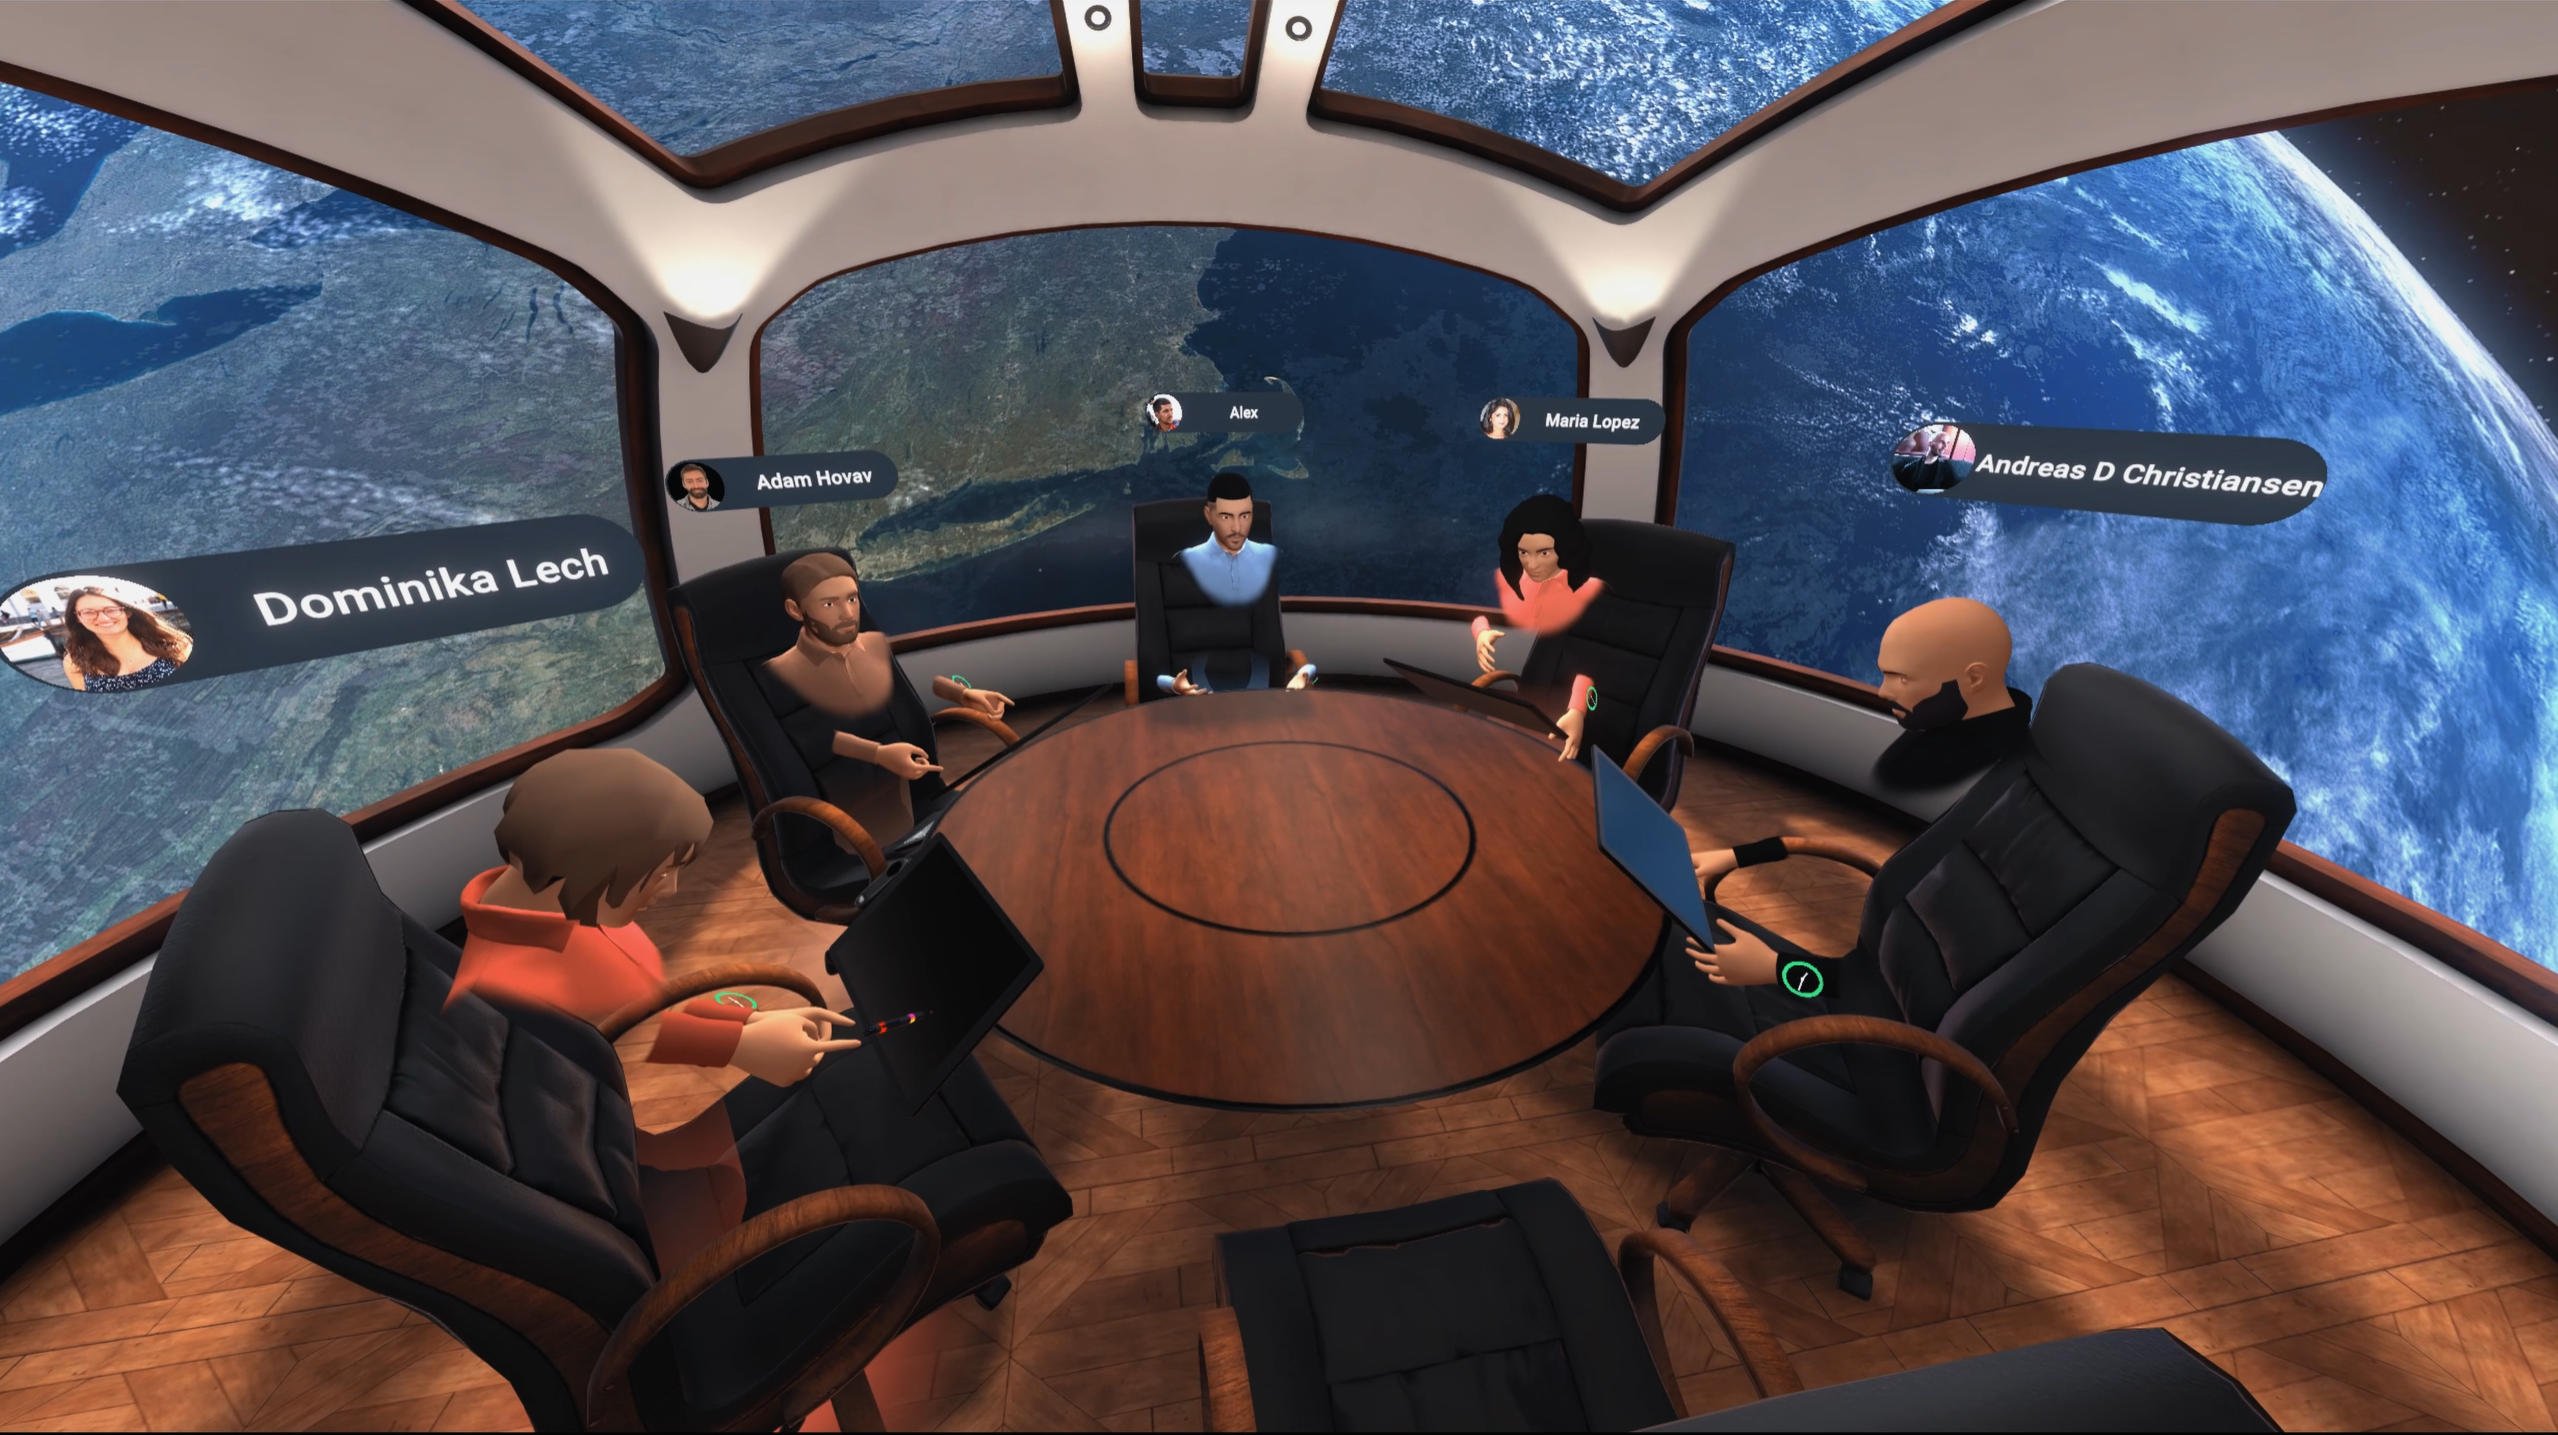
\includegraphics[width=\textwidth]{images/meetinvr_vr_conference.png}
	\caption{Example of environment in a VR event platform.}
	\label{figure:motivation-vr}
\end{figure}

This platform offers the most immersion there is but it also comes with a steeper learning curve because not many users have interacted with VR headsets and controllers compared to the ubiquitous keyboard and mouse as used in 3D environments, what is even worse is that you are required to own a VR device and a capable machine. Furthermore the users have to go through the process of setting up the device and the chances are low of running this on mobile. \\

\subsection*{Conclusion}
After examining the platforms that provide virtual events I have come to the conclusion that most of them are not user friendly and require learning steps. Additionally, the applications in both categories can share disadvantages such as:
\begin{itemize}
    \item May require development of distinct desktop and mobile applications (as a consequence the application may not work on certain operating systems).
    \item May require download of big files and lengthy installation time.
    \item From the developer's point of view, may assume application maintenance overhead such as updating it, developing patches, and upgrading. The updates then need to be made available to the end users, in case the user doesn't run the update then there can appear inconsistency, usability and security problems.
\end{itemize}

The solution is to build a virtual event platform that: requires few learning steps,	 is easily accessible across devices, has few maintenance headaches and is always up-to-date. That is an application which is intuitive to use and it \textbf{just works}.

